\documentclass[11pt,a4paper]{article}
\usepackage[utf8]{inputenc}
\usepackage[T1]{fontenc}
\usepackage[brazil]{babel}
\usepackage[margin=2.5cm]{geometry}
\usepackage{booktabs}
\usepackage{amsmath,amssymb}
\usepackage{caption}
\usepackage{graphicx}
\usepackage{setspace}
\usepackage{enumitem}
\usepackage{placeins}
\usepackage{longtable}
\usepackage{float}
\usepackage[hidelinks]{hyperref}
\graphicspath{{v2 OFICIAL/figuras/}}
\setstretch{1.4}
\captionsetup{font=small,labelsep=colon}
\setcounter{tocdepth}{2}

\title{Peso de VALE3 nos fundos de investimento brasileiros:\\
um modelo de fator dinâmico com correção logística e ajuste parcial}
\author{João Paulo Zangrandi\\
Fundação Getulio Vargas --- Escola de Economia de São Paulo (FGV--EESP)\\
Orientador: Prof.\ Mauricio Ferraresi}
\date{}

\begin{document}
\maketitle

\tableofcontents
\newpage

% ======================================================================
\section{Introdução}

\emph{[Seção a ser escrita por último.]}

% ======================================================================
\section{Revisão de literatura}

\emph{[Seção a ser desenvolvida após indicação de referências pelo orientador. Áreas de
inserção previstas: precificação de ativos baseada em demanda (\emph{demand-based asset
pricing}); comportamento de fundos de investimento e efeitos de fluxo; modelos de ajuste
parcial em finanças corporativas e de portfólio.]}

% ======================================================================
\section{Dados}
\label{sec:dados}

\FloatBarrier
\subsection{Fontes e universo}

Os dados vêm de dois registros públicos que a CVM exige de todo fundo de investimento
brasileiro: a Composição e Diversificação de Aplicações (CDA), extrato mensal de que vem o peso
de cada ativo na carteira de cada fundo (a variável dependente deste trabalho), e o Informe
Diário, de onde vêm patrimônio líquido, cotistas, captação e resgate (as características do
fundo). O período coberto vai de janeiro de 2016 a dezembro de 2021. O universo de fundos parte
de todo fundo do universo CVM que já teve VALE3 em carteira em algum momento do período (2.820
fundos, 41 grupos de gestora por marca controladora), e para esses fundos observa-se \textbf{toda
ação} que carregam, não só VALE3.

\begin{table}[h]\centering\small
\caption{Evolução do universo de dados. Fonte: scripts \texttt{17}--\texttt{29} $\to$
\texttt{painel\_multiativo\_final.csv}.}
\label{tab:universo}
\begin{tabular}{@{}p{6.4cm}rrrr@{}}
\toprule
Etapa & Universo (fundos) & Amostra final (fundos) & Gestoras & Ativos \\
\midrule
Ampliação de gestoras (todo o universo CVM, só VALE3) & 2.820 & 2.295 & 41 & 1 \\
Ampliação de ativos (todo o universo CVM, todas as ações) & 2.820 & 2.347 & 41 & 501 \\
\bottomrule
\end{tabular}
\caption*{\footnotesize Amostra final = fundos com as 6 características (Seção~\ref{sec:dados})
simultaneamente disponíveis em pelo menos um mês. A cobertura temporal efetiva é de 59 meses
(fev/2017--dez/2021, não os 72 meses do período bruto): o beta do fundo exige 252 pregões de
histórico de cota, o que exclui os primeiros 12 meses da amostra.}
\end{table}

Dos 473 fundos do universo bruto que não entram na amostra final, 28 nunca têm as quatro
características do Informe Diário completas ao mesmo tempo; os outros 445 têm essas quatro, mas
nunca chegam a ter beta --- 91,2\% deles (406) simplesmente não acumulam 252 dias de cota válida
na janela 2016--2021 (fundos jovens demais, não uma limitação de dado), 4,0\% (18) acumulam mas
começam tarde demais para deixar mês seguinte disponível como preditor, e só 4,7\% (21) têm um
padrão mais consistente com fechamento do fundo.

\FloatBarrier
\subsection{Limpeza e características}

Um mesmo ativo pode aparecer na CDA sob rótulos diferentes conforme o tipo de posição (direta,
cedida/recebida em empréstimo, direito de subscrição). Este trabalho mantém apenas a posição
direta, identificada pelo sufixo numérico do código de negociação (convenção B3: sufixos 3, 4,
5, 6, 7, 8, 11) --- 523 ativos de posição direta, 10.603.928 linhas de fundo-ativo-mês antes dos
demais filtros.

Seis características de cada fundo entram no modelo (equação~\eqref{eq:cs}), todas medidas no
último dia do mês anterior ao da observação, para evitar viés de antecipação:

\begin{table}[h]\centering\small
\caption{As 6 características da Etapa 1. Fonte: Informe Diário da CVM (5 primeiras) e
\texttt{painel\_multiativo\_final.csv} (HHI\_resto, derivado do próprio peso).}
\label{tab:caracteristicas}
\begin{tabular}{@{}p{2.6cm}p{9.5cm}@{}}
\toprule
Característica & Definição \\
\midrule
Tamanho & Logaritmo do patrimônio líquido \\
Cotistas & Logaritmo do número de cotistas \\
FIC & Indicador (0/1) de ser fundo de cotas de outro fundo \\
Fluxo/AUM & (Captação $-$ resgate) sobre o patrimônio líquido \\
Beta do fundo & Covariância do retorno diário da cota com o Ibovespa / variância do Ibovespa,
janela móvel de 252 pregões \\
$\text{HHI}_{\text{resto}}$ & Concentração do restante da carteira de ações, excluindo o
ativo-alvo (equação~\eqref{eq:hhi-resto}) --- calculado sobre o sub-portfólio de ações capturado
neste painel (não o NAV inteiro do fundo, que também pode incluir renda fixa e caixa não
observados aqui) \\
\bottomrule
\end{tabular}
\end{table}

\FloatBarrier
\subsection{Amostra final}

\begin{table}[h]\centering
\caption{Dimensões da amostra final. Fonte: \texttt{painel\_multiativo\_final.csv}.}
\label{tab:amostra}
\begin{tabular}{@{}lr@{}}
\toprule
Observações (fundo $\times$ ativo $\times$ mês) & 8.268.920 \\
Fundos & 2.347 \\
Grupos de gestora & 41 \\
Ativos (posição direta) & 501 \\
Meses (fev/2017--dez/2021) & 59 \\
\bottomrule
\end{tabular}
\caption*{\footnotesize Esta é a base única usada em toda a Seção~\ref{sec:resultados} --- ao
contrário da versão anterior deste documento, não há troca de base entre Etapas.}
\end{table}

% ======================================================================
\section{Metodologia}
\label{sec:metodologia}

O trabalho é organizado em três etapas sequenciais, cada uma alimentando a seguinte. A primeira
etapa estima, mês a mês, o peso que cada fundo \emph{deveria} carregar em cada ativo, dadas as
características observáveis do fundo. A segunda etapa modela a velocidade com que o peso
efetivamente observado converge a esse alvo. A terceira etapa testa, em dados que o modelo nunca
viu durante a estimação, se essa modelagem tem valor preditivo genuíno. Em cada uma das três
etapas, o erro é o principal objeto de análise: sua estrutura (quem erra mais, quando, e em que
direção) é o que permite comparar fundos e gestoras entre si.

\FloatBarrier
\subsection{Etapa 1: cross-section}

Para cada ativo $n$ e cada mês $t$, o peso que um fundo $i$ carrega é modelado como função
logística de seis características do fundo:
\begin{equation}
\text{peso}_{i,n,t} = g\big(x_{i,n,t}'\theta_{n,t}\big) + e_{i,n,t}, \qquad
g(z) = \frac{1}{1+e^{-z}}
\label{eq:cs}
\end{equation}
em que $x_{i,n,t}$ reúne seis características do fundo (Seção~\ref{sec:dados}): tamanho (log
AUM), número de cotistas (log), indicador de fundo de cotas (FIC), fluxo de captação/resgate
sobre o patrimônio, beta do próprio fundo, e a concentração do restante da carteira ($\text{HHI}_{\text{resto}}$,
definida na equação~\eqref{eq:hhi-resto} abaixo) --- todas padronizadas, exceto o indicador de
FIC. $\theta_{n,t}$ é o vetor de coeficientes daquele ativo naquele mês, estimado por máxima
verossimilhança (regressão logística quase-binomial), separadamente para cada célula
(ativo, mês) com número mínimo de fundos detentores, sem nenhuma etapa de agregação temporal por
cima: cada $\theta_{n,t}$ é o resultado de uma única regressão de corte transversal.

\begin{equation}
\text{HHI}_{\text{resto},i,n,t} = \sum_{m \neq n} \text{peso}_{i,m,t}^2 =
\underbrace{\sum_{m} \text{peso}_{i,m,t}^2}_{\text{HHI}_{\text{total}}} - \text{peso}_{i,n,t}^2
\label{eq:hhi-resto}
\end{equation}
$\text{HHI}_{\text{resto}}$ mede a concentração da carteira de ações do fundo $i$ no mês $t$,
\textbf{excluindo o próprio ativo-alvo} $n$ --- excluir $n$ evita a circularidade óbvia de usar a
concentração de uma carteira que já inclui o peso que se está tentando explicar como variável
explicativa dele mesmo. Um piloto com amostra aleatória de 100 células (ativo, mês), sem viés de
seleção, mostrou efeito forte e consistente antes de essa característica ser incorporada à
especificação principal: 77\% das células com coeficiente padronizado significativo, sinal
positivo em 75 das 77, ganho médio de pseudo-$R^2$ de $0{,}080$.

O erro dessa etapa, $e_{i,n,t} = \text{peso}_{i,n,t} - g(x_{i,n,t}'\theta_{n,t})$, mede o quanto
a posição observada de um fundo se afasta do que suas próprias características explicam,
\emph{dentro} do mesmo mês. Por construção da máxima verossimilhança, a média desse erro é
mecanicamente zero em cada célula --- não é evidência de bom ajuste, apenas uma propriedade
algébrica do estimador. O que de fato varia, e é informativo, é a dispersão do erro.

\FloatBarrier
\subsection{Etapa 2: ajuste parcial}

A Etapa 1 estima um alvo, $w^*_{i,n,t} = g(x_{i,n,t}'\theta_{n,t})$, mas não diz nada sobre a
\emph{dinâmica}: quão rápido a posição real de um fundo converge a esse alvo, mês a mês. A
segunda etapa modela essa dinâmica através de um mecanismo de ajuste parcial: a cada mês, o
fundo fecha uma fração $\lambda$ da distância entre sua posição atual e o alvo.
\begin{equation}
w_{i,n,t+1} - w_{i,n,t} = \lambda\, d_{i,n,t} + u_{i,n,t+1}, \qquad
d_{i,n,t} \equiv w^*_{i,n,t} - w_{i,n,t}
\label{eq:pa}
\end{equation}
$\lambda$ é estimado por mínimos quadrados ordinários diretos, sem intercepto, com todos os
pares de meses consecutivos agrupados (\emph{pooled}) --- um único coeficiente, a mesma
velocidade de ajuste para todo fundo e todo ativo.

\FloatBarrier
\subsection{Etapa 3: esquema fora da amostra}

As duas primeiras etapas são estimadas com a amostra inteira e, por isso, não dizem se o modelo
tem valor preditivo de verdade. A terceira etapa testa isso diretamente, com um corte temporal
único: o parâmetro $\lambda_h$, para cada horizonte $h$, é reestimado usando \textbf{apenas} os
meses de treino, anteriores a janeiro de 2020, e então aplicado, fixo, aos meses de teste, de
janeiro de 2020 em diante --- período que o modelo nunca viu durante a estimação.
\begin{align}
\widehat w_{i,n,t+h} &= w_{i,n,t} + \widehat\lambda_{h,\text{treino}}\, d_{i,n,t}
&&\text{(ajuste parcial)} \notag\\
\widehat w_{i,n,t+h} &= w_{i,n,t} &&\text{(previsão ingênua)}
\label{eq:oos}
\end{align}
O erro fora da amostra, $\text{erro}_{i,n,t+h} = \big(w_{i,n,t+h}-w_{i,n,t}\big) -
\widehat\lambda_{h,\text{treino}}\, d_{i,n,t}$, é comparado ao erro da previsão ingênua (que
simplesmente assume que nada muda) através da raiz do erro quadrático médio (RMSE). A diferença
percentual entre os dois RMSEs (\textbf{margem}) responde à pergunta central: o ajuste parcial
estimado com dados antigos ainda ajuda a prever dados novos, ou uma previsão ingênua seria tão
boa quanto?

\FloatBarrier
\subsection{Extensões}

O procedimento --- Etapas 1 a 3 --- é aplicado a todas as gestoras do universo CVM e a todas as
ações que essas gestoras carregam, repetindo a equação~\eqref{eq:cs} célula por célula de
ativo-mês. A Etapa 3 é igualmente generalizada: o índice de ativo $n$ e o horizonte $h$ são
explícitos na equação~\eqref{eq:pa}, permitindo agregar o erro fora da amostra por gestora, por
ativo e por horizonte de previsão simultaneamente.

% ======================================================================
\section{Resultados}
\label{sec:resultados}

Toda esta seção usa a base multiativo (Tabela~\ref{tab:amostra}: 2.343 fundos, 41 gestoras, 501
ativos, após excluir 597 fundo-mês com soma de peso $>105\%$ do patrimônio --- erro de reporte
identificado na CDA da CVM, não deste trabalho) --- uma única base do início ao fim, diferente de
versões anteriores deste documento.

\FloatBarrier
\subsection{Etapa 1: cross-section}

O modelo (equação~\eqref{eq:cs}) é estimado célula a célula (ativo, mês); 13.925 células
convergiram (21 não convergiram, excluídas). A Tabela~\ref{tab:theta} resume o coeficiente
padronizado (log-odds) e a Tabela~\ref{tab:ape} o efeito marginal médio (APE, pontos percentuais)
de cada característica, entre as 13.925 células.

\begin{table}[h]\centering\small
\caption{Coeficiente padronizado (log-odds) de cada característica, mediana e \% de células com
sinal positivo, entre 13.925 células (ativo, mês). Fonte: script \texttt{97\_theta\_ape\_hhi.R}
$\to$ \texttt{theta\_multiativo.csv}.}
\label{tab:theta}
\begin{tabular}{@{}lrr@{}}
\toprule
Característica & Mediana & \% de células positivo \\
\midrule
Tamanho ($\theta^{aum}$) & $-0{,}0167$ & $46{,}8\%$ \\
Cotistas ($\theta^{cot}$) & $0{,}1206$ & $70{,}9\%$ \\
Fundo de cotas ($\theta^{fic}$) & $0{,}0199$ & $51{,}7\%$ \\
Fluxo/AUM ($\theta^{flow}$) & $0{,}0559$ & $54{,}1\%$ \\
Beta do fundo ($\theta^{bf}$) & $0{,}7242$ & $85{,}3\%$ \\
$\text{HHI}_{\text{resto}}$ ($\theta^{hhi}$) & $0{,}4950$ & $87{,}3\%$ \\
\bottomrule
\end{tabular}
\caption*{\footnotesize Pseudo-$R^2$ de McFadden médio (com piso em $-1$, ver nota do script): $0{,}526$.
$\text{HHI}_{\text{resto}}$ é significativo ($|t|>1{,}96$) em $72{,}9\%$ das células ($10.145$ de
$13.925$), com sinal positivo em $95{,}4\%$ dos casos significativos --- concentrar o restante da
carteira aumenta a probabilidade de concentrar também no ativo-alvo.}
\end{table}

\begin{table}[h]\centering\small
\caption{Efeito marginal médio (APE, pontos percentuais de peso), mesma base da Tabela~\ref{tab:theta}.
Fonte: script \texttt{97\_theta\_ape\_hhi.R} $\to$ \texttt{theta\_multiativo.csv}.}
\label{tab:ape}
\begin{tabular}{@{}lrr@{}}
\toprule
Característica & Mediana (p.p.) & \% de células positivo \\
\midrule
Tamanho & $-0{,}0002\%$ & $46{,}8\%$ \\
Cotistas & $0{,}0094\%$ & $70{,}9\%$ \\
Fundo de cotas & $0{,}0001\%$ & $51{,}6\%$ \\
Fluxo/AUM & $0{,}0034\%$ & $54{,}1\%$ \\
Beta do fundo & $0{,}0992\%$ & $85{,}3\%$ \\
$\text{HHI}_{\text{resto}}$ & $0{,}0515\%$ & $87{,}3\%$ \\
\bottomrule
\end{tabular}
\end{table}

\begin{table}[h]\centering\small
\caption{Estatísticas do erro $e$, Etapa 1, 8.208.201 observações. Fonte: script
\texttt{96\_pipeline\_hhi\_etapa1.R} $\to$ \texttt{erro\_e\_multiativo.csv}.}
\label{tab:erro-e}
\begin{tabular}{@{}lr@{}}
\toprule
Estatística & Valor \\
\midrule
Média & $0{,}000000$ \\
Desvio-padrão & $0{,}0105$ \\
Mediana & $-0{,}0003$ \\
Mínimo / Máximo & $-0{,}658$ / $0{,}988$ \\
\% de observações com $e>0$ & $26{,}1\%$ \\
Assimetria & $7{,}05$ \\
Curtose & $436{,}19$ (normal $=3$) \\
Previsões fora de $[0,1]$ & $0$ de $8.208.201$ \\
\bottomrule
\end{tabular}
\caption*{\footnotesize Assimetria/curtose bem mais altas que na versão de 1 ativo (VALE3--Itaú)
--- esperado: a base multiativo mistura 501 ativos de liquidez e perfil muito diferentes numa
única distribuição agregada.}
\end{table}

\FloatBarrier
\subsection{Etapa 2: ajuste parcial}

$\lambda$ (equação~\eqref{eq:pa}) estimado por MQO \emph{pooled}, todos os pares de meses
consecutivos, toda a amostra: $\widehat\lambda = 0{,}0779$.

\begin{table}[h]\centering\small
\caption{Estatísticas do erro $u$, Etapa 2, 7.447.629 pares de meses consecutivos. Fonte: script
\texttt{98\_etapa1\_etapa2\_stats\_multiativo.R} $\to$ \texttt{erro\_u\_multiativo.csv}.}
\label{tab:erro-u}
\begin{tabular}{@{}lr@{}}
\toprule
Estatística & Valor \\
\midrule
Média & $-0{,}00003$ \\
Desvio-padrão & $0{,}0043$ \\
Mediana & $-0{,}00003$ \\
Mínimo / Máximo & $-0{,}611$ / $0{,}592$ \\
\% de observações com $u>0$ & $33{,}4\%$ \\
Assimetria & $0{,}71$ \\
Curtose & $521{,}20$ (normal $=3$) \\
\bottomrule
\end{tabular}
\end{table}

\FloatBarrier
\subsection{Etapa 3: esquema fora da amostra}

$\lambda_h$ (equação~\eqref{eq:oos}) estimado só em treino ($<$jan/2020), aplicado fixo ao teste
(jan/2020--dez/2021). A Tabela~\ref{tab:oos-agregado} traz o RMSE agregado nos 4 horizontes, e
compara diretamente o modelo com 6 características (com $\text{HHI}_{\text{resto}}$) contra a
versão anterior de 5 características.

\begin{table}[h]\centering\small
\caption{RMSE fora da amostra, ajuste parcial vs.\ previsão ingênua, 4 horizontes --- com e sem
$\text{HHI}_{\text{resto}}$ na Etapa 1. Fonte: script \texttt{96\_pipeline\_hhi\_etapa1.R} (6
caract.) e \texttt{comparacao\_hhi\_vs\_original.csv} (comparação).}
\label{tab:oos-agregado}
\begin{tabular}{@{}lrrrr@{}}
\toprule
& $h=1$ & $h=3$ & $h=6$ & $h=12$ \\
\midrule
RMSE ajuste parcial (6 características) & $0{,}003856$ & $0{,}005610$ & $0{,}006804$ & $0{,}008179$ \\
RMSE previsão ingênua & $0{,}003922$ & $0{,}005813$ & $0{,}007177$ & $0{,}008828$ \\
Razão ajuste/ingênua & $0{,}9830$ & $0{,}9651$ & $0{,}9481$ & $0{,}9265$ \\
\midrule
RMSE ajuste parcial (5 características, sem HHI) & $0{,}003859$ & $0{,}005619$ & --- & --- \\
Variação ao incluir $\text{HHI}_{\text{resto}}$ & $-0{,}073\%$ & $-0{,}156\%$ & --- & --- \\
\bottomrule
\end{tabular}
\caption*{\footnotesize $\lambda_1=0{,}0793$, $\lambda_3=0{,}1689$, $\lambda_6=0{,}2513$,
$\lambda_{12}=0{,}3818$. A melhora com HHI é pequena mas consistente nos dois horizontes
comparados diretamente --- efeito principal do HHI está em \emph{quem} erra mais/menos
(adiante), não no RMSE agregado.}
\end{table}

\begin{table}[h]\centering\small
\caption{$\lambda$ fixo (treino único) vs.\ janela expansiva (reestimado mês a mês, sem
vazamento), fora da amostra, $h=1$, base multiativo (6 características). Fonte: script
\texttt{82\_etapa3\_multiativo\_janela\_expansiva.R}.}
\label{tab:janela_expansiva}
\begin{tabular}{@{}p{5.2cm}rrr@{}}
\toprule
Meses de teste & $\lambda$ fixo & $\lambda$ expansiva \\
\midrule
23 & $0{,}9830$ & $0{,}9831$ \\
\bottomrule
\end{tabular}
\caption*{\footnotesize Razão RMSE/RMSE ingênua. Ambas as versões vencem a ingênua em 23 dos 23
meses; correlação de Spearman do ranking de dificuldade por gestora entre as duas versões de
$\lambda$: $1{,}0000$. Confirma a robustez do $\lambda$ fixo já vista na versão anterior deste
documento.}
\end{table}

\begin{figure}[H]\centering
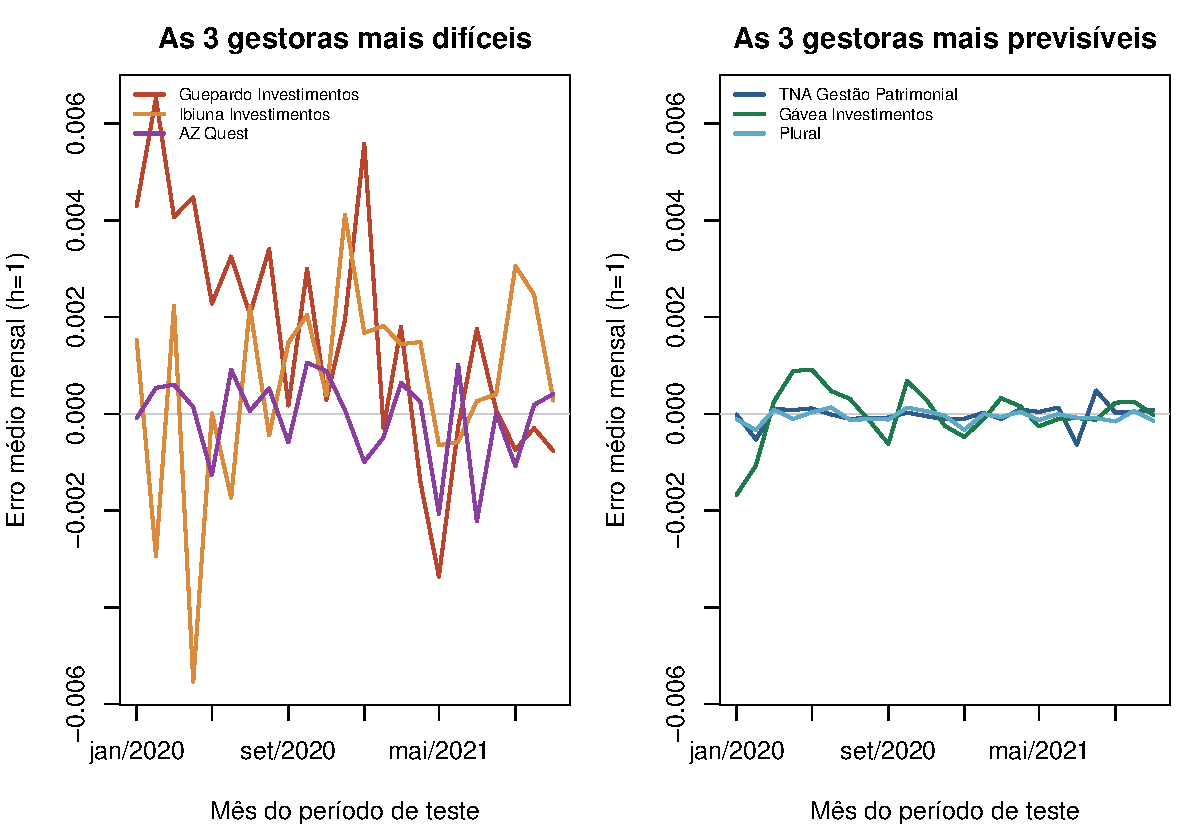
\includegraphics[width=0.95\textwidth]{fig_dinamica_erro_gestora_extremos.pdf}
\caption{Evolução mensal do erro médio fora da amostra ($h=1$), 3 gestoras mais difíceis e 3 mais
previsíveis (Tabelas~\ref{tab:rmse-gestora}--\ref{tab:margem-gestora}). Fonte: script
\texttt{74\_figuras\_dinamica\_erro\_tcc.R} $\to$ \texttt{etapa3\_multiativo\_h1.csv}.}
\end{figure}

\begin{figure}[H]\centering
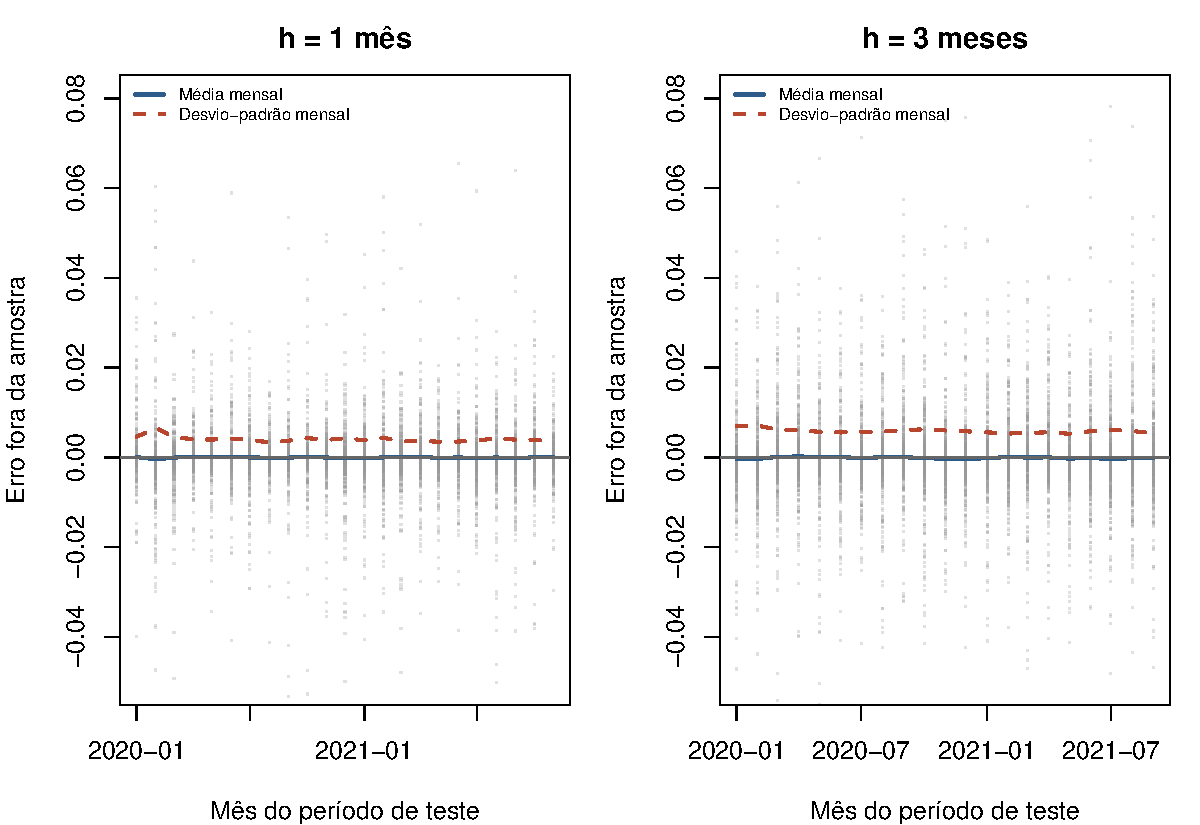
\includegraphics[width=0.95\textwidth]{fig_dinamica_erro_oos_agregado.pdf}
\caption{Erro fora da amostra agregado (nuvem cinza: individual; azul: média mensal; vermelho:
desvio-padrão mensal). Esquerda: $h=1$; direita: $h=3$. Fonte: script
\texttt{74\_figuras\_dinamica\_erro\_tcc.R}.}
\end{figure}

\begin{figure}[H]\centering
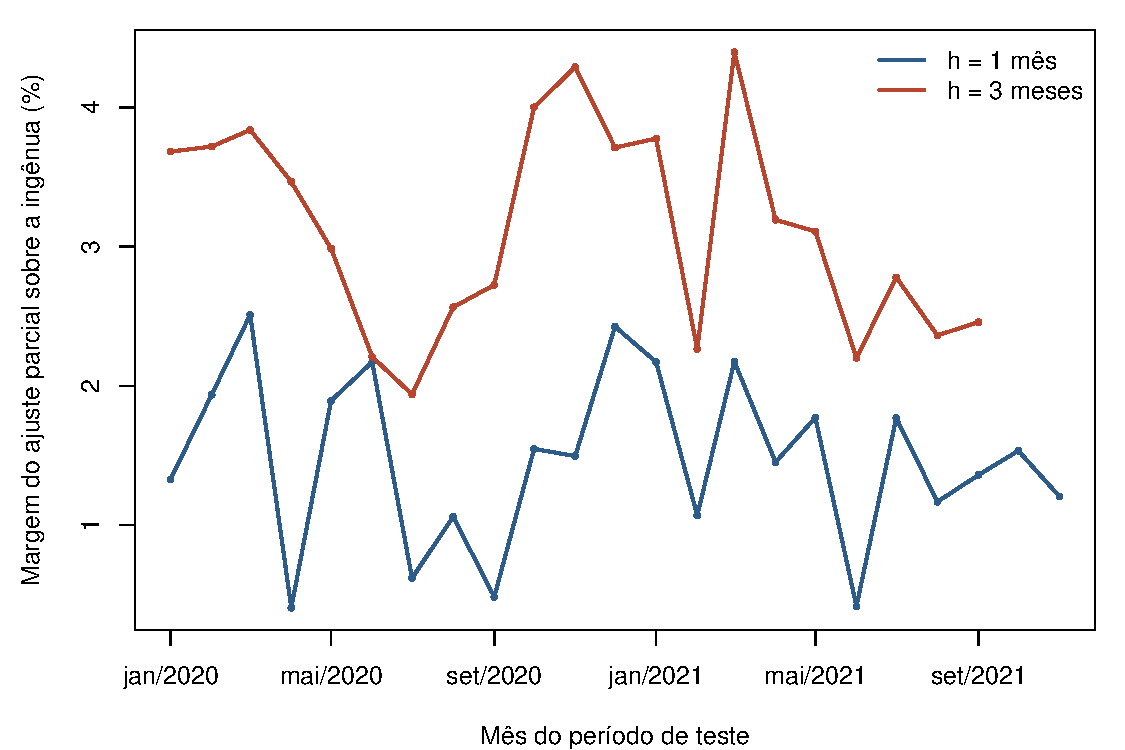
\includegraphics[width=0.75\textwidth]{fig_margem_dinamica_mensal.pdf}
\caption{Margem do ajuste parcial sobre a ingênua, mês a mês ($h=1$: média $1{,}63\%$; $h=3$:
média $3{,}46\%$). Fonte: script \texttt{75\_figura\_margem\_dinamica.R}.}
\end{figure}

\begin{figure}[H]\centering
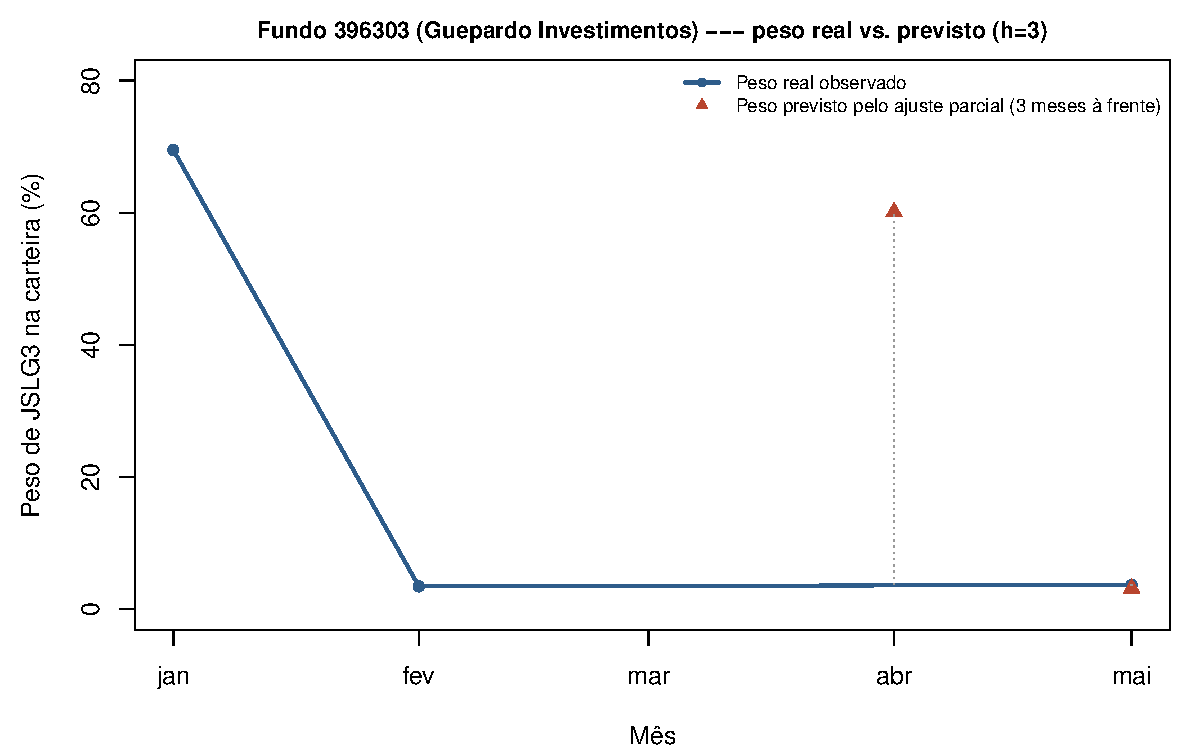
\includegraphics[width=0.78\textwidth]{fig_trajetoria_fundo_guepardo_jslg3.pdf}
\caption{Peso real vs.\ previsto ($h=3$), fundo 396303 (Guepardo Investimentos), JSLG3 --- ainda o
fundo com maior RMSE fora da amostra mesmo com HHI incluído. Desmonte de posição concentrada
($69{,}5\%\to3{,}8\%$ do patrimônio entre jan/2020 e fev/2020) que o modelo não antecipa. Fonte:
script \texttt{92\_figura\_trajetoria\_fundo\_v2.R}.}
\label{fig:trajetoria-fundo}
\end{figure}

\begin{figure}[H]\centering
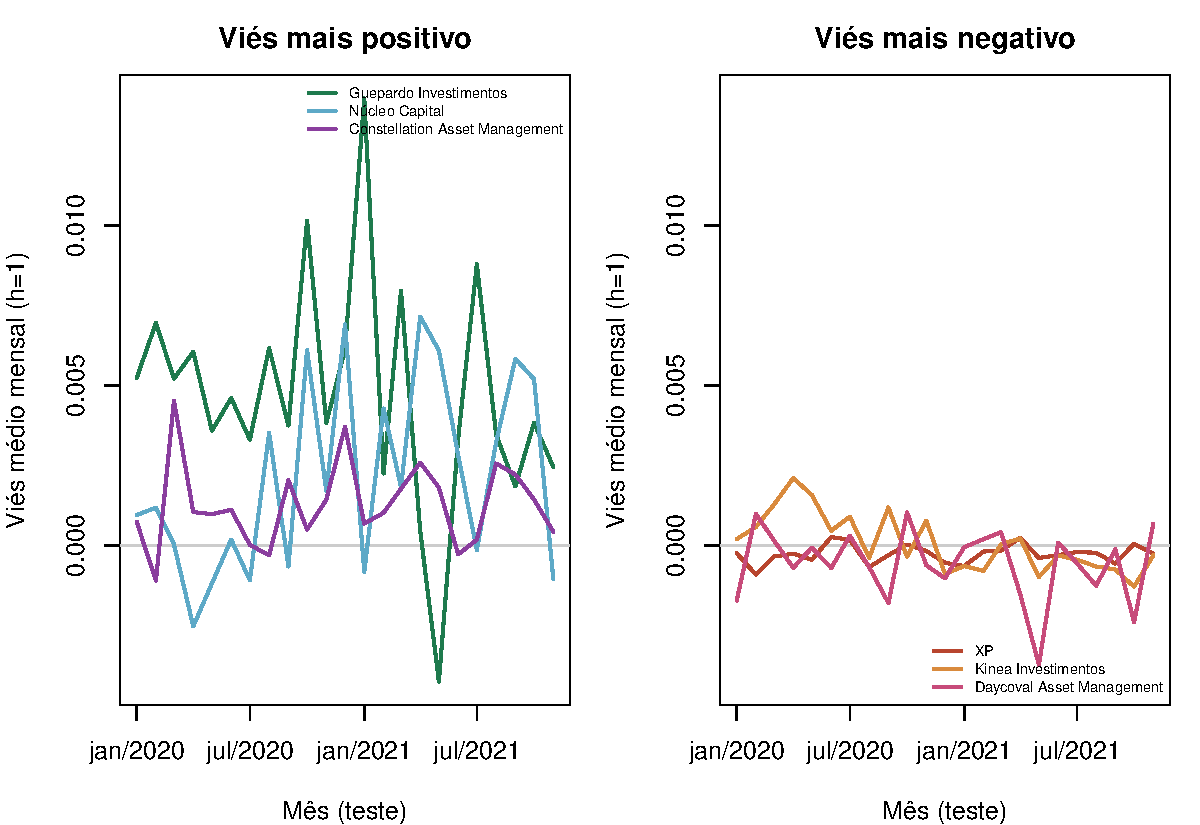
\includegraphics[width=0.95\textwidth]{fig_vies_dinamico_gestora.pdf}
\caption{Viés médio mensal fora da amostra, com sinal, 3 gestoras mais positivas e 3 mais
negativas (mín.\ 100 obs.\ de teste). Maior viés positivo: Guepardo ($0{,}00356$), Núcleo Capital
($0{,}00186$); maior negativo: Daycoval ($-0{,}00067$), Kinea ($-0{,}00034$). Fonte: script
\texttt{77\_figura\_vies\_dinamico\_gestora.R}.}
\label{fig:vies-dinamico}
\end{figure}

\paragraph{Persistência do viés.} Dividindo os 23 meses de teste ao meio: correlação de
$0{,}71$ ($R^2=0{,}50$) entre o viés médio de cada gestora nas duas metades --- persistente, um
pouco menos que na versão sem HHI ($0{,}80$), consistente com HHI absorvendo parte do que antes
aparecia como viés sistemático de gestora.

\begin{figure}[H]\centering
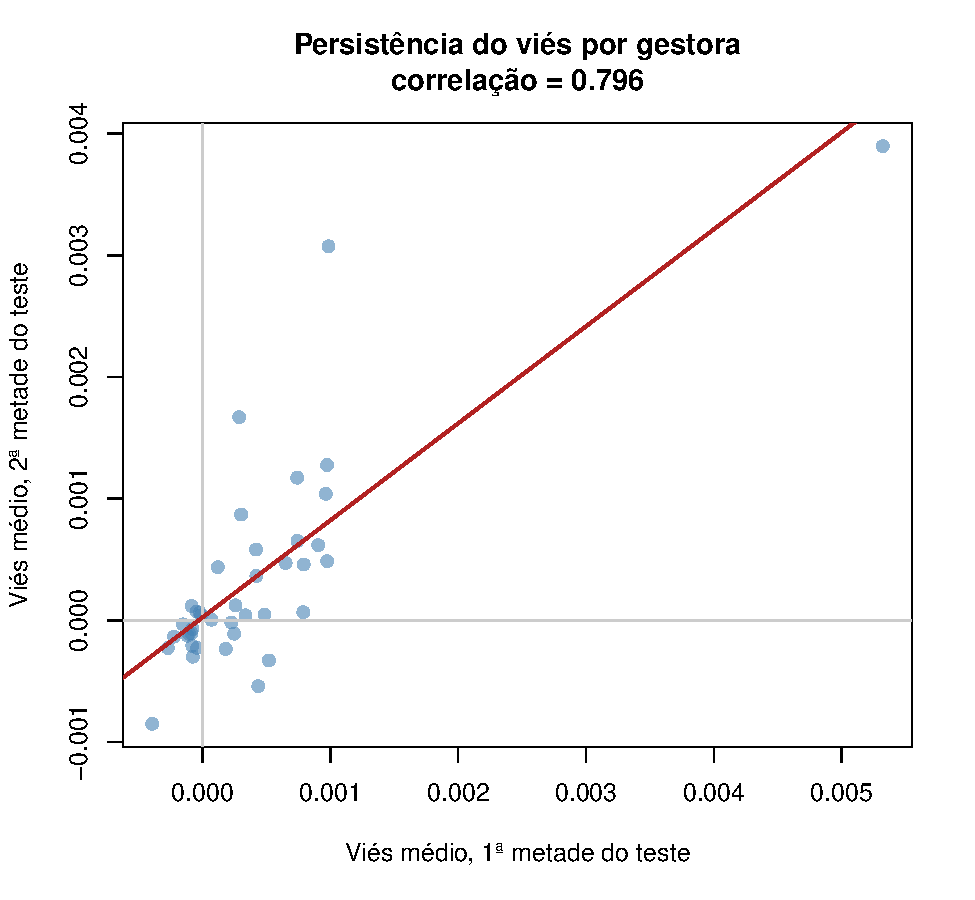
\includegraphics[width=0.55\textwidth]{fig_persistencia_vies_gestora.pdf}
\caption{Viés médio, 1ª metade do teste (2020) vs.\ 2ª metade (2021), 40 gestoras. Fonte: script
\texttt{84\_persistencia\_vies\_gestora.R}.}
\label{fig:persistencia-vies}
\end{figure}

\paragraph{Correção de viés.} Estimando o viés na 1ª metade e aplicando-o, fixo, à 2ª: RMSE cai de
$0{,}005699$ para $0{,}005697$ --- melhora de $0{,}04\%$ (era $0{,}07\%$ sem HHI), irrelevante na
prática.

\paragraph{Decomposição $\text{RMSE}^2=\text{viés}^2+\text{variância}$.} Em média entre as 40
gestoras, viés$^2$ explica $0{,}59\%$ do $\text{RMSE}^2$ (mediana $0{,}15\%$; máximo $3{,}64\%$,
Real Investor). \emph{Pooled} (todas as observações juntas): $0{,}001\%$. A variância domina.

\begin{figure}[H]\centering
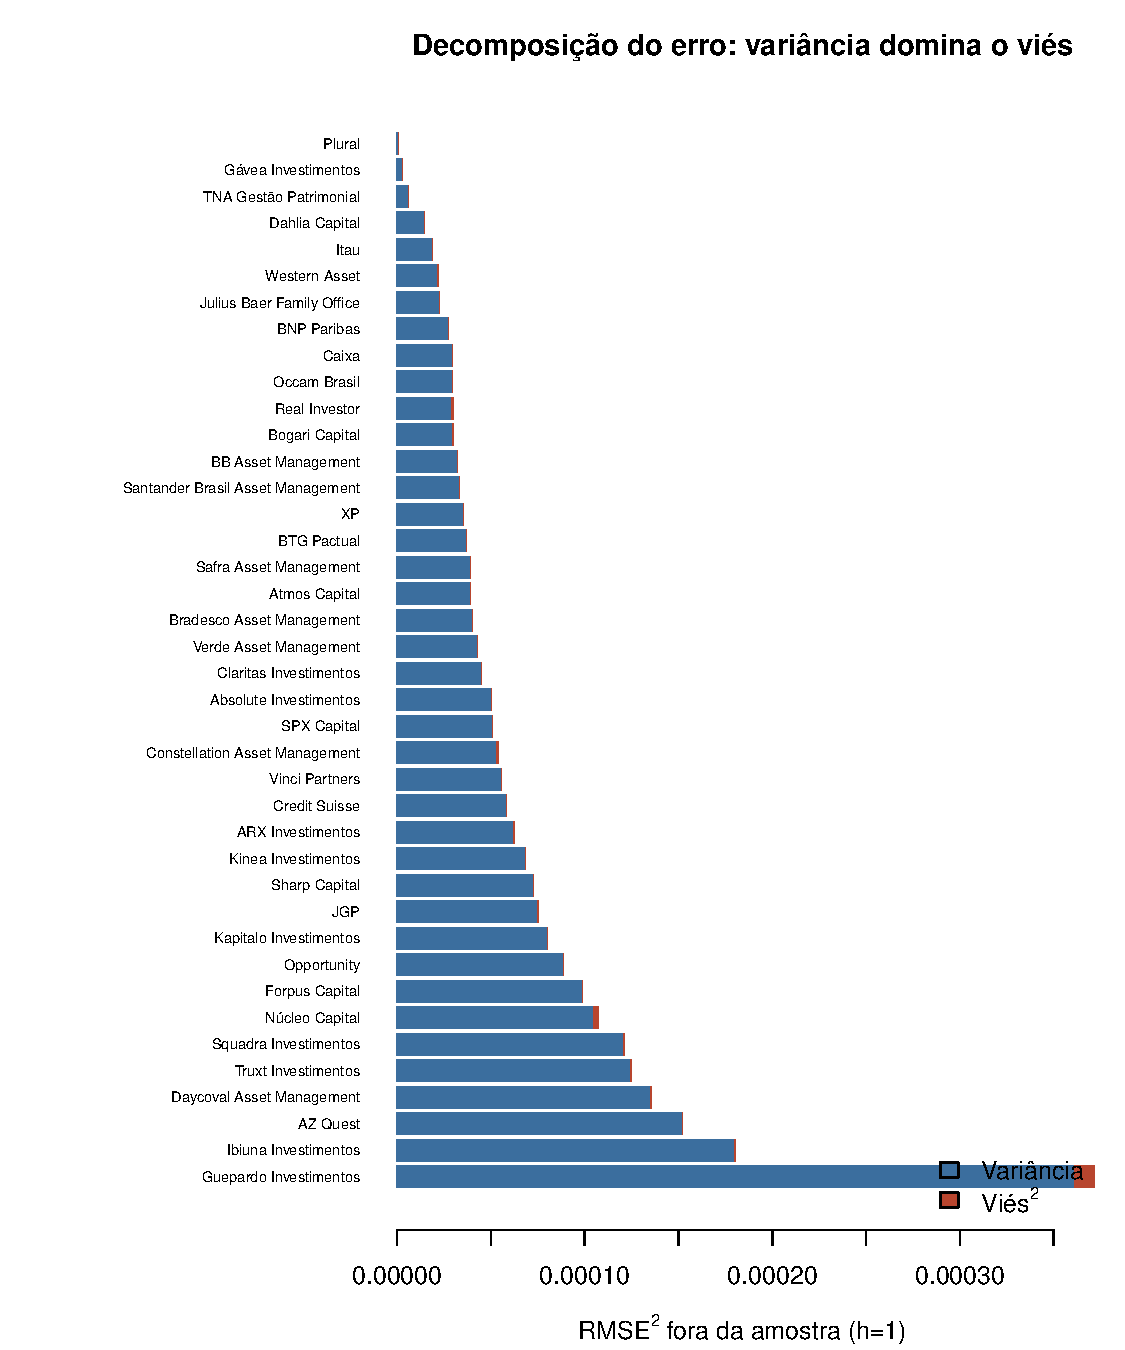
\includegraphics[width=0.68\textwidth]{fig_decomposicao_vies_variancia.pdf}
\caption{Decomposição do erro fora da amostra ($h=1$) por gestora, ordenada por RMSE. Fonte:
script \texttt{86\_decomposicao\_e\_persistencia\_variancia.R}.}
\label{fig:decomposicao-vies-variancia}
\end{figure}

\paragraph{Persistência da variância.} Correlação de $0{,}85$ ($R^2=0{,}72$) entre o
desvio-padrão do erro na 1ª e na 2ª metade do teste --- tão persistente quanto na versão sem HHI
($0{,}85$, $R^2=0{,}71$): HHI não absorve a persistência da variância como absorveu parte da do
viés.

\begin{figure}[H]\centering
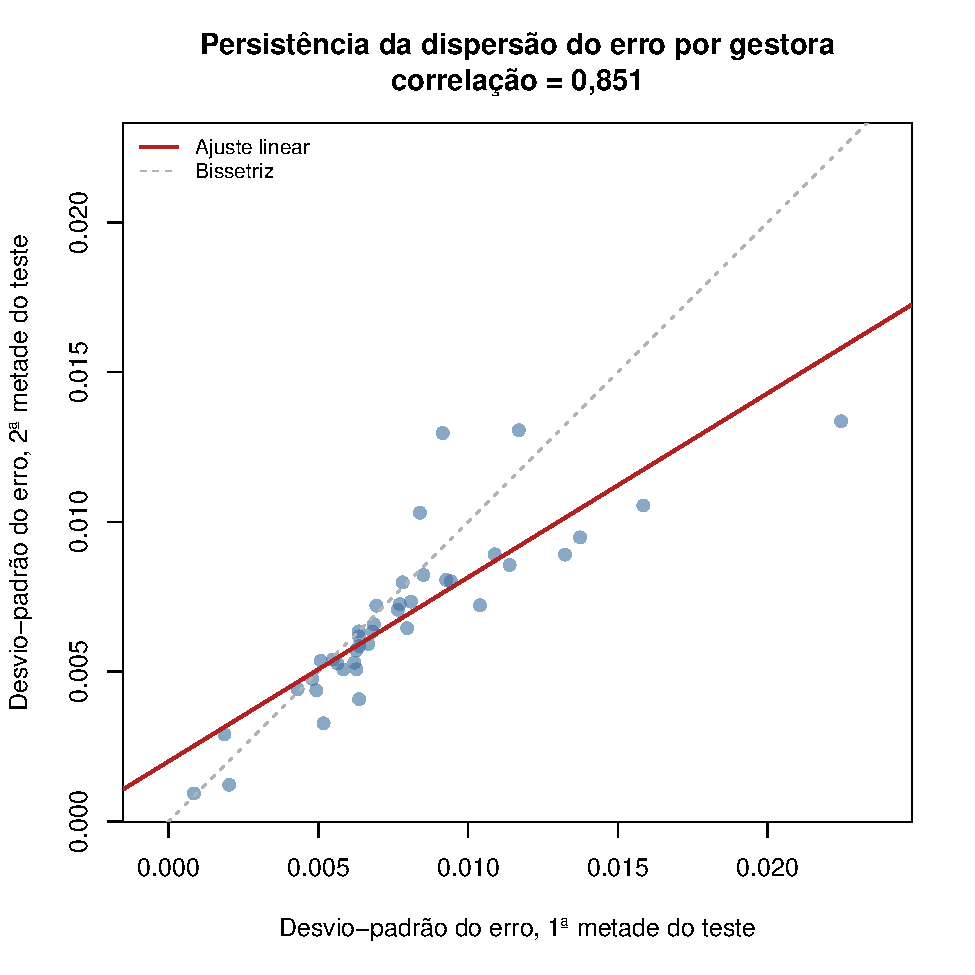
\includegraphics[width=0.55\textwidth]{fig_persistencia_dp_gestora.pdf}
\caption{Desvio-padrão do erro, 1ª vs.\ 2ª metade do teste, 40 gestoras. Linha tracejada: $y=x$.
Fonte: script \texttt{86\_decomposicao\_e\_persistencia\_variancia.R}.}
\label{fig:persistencia-dp}
\end{figure}

\paragraph{O que explica a variância.} Duas construções de concentração aparecem neste trabalho:
$\text{HHI}_{\text{resto}}$ (equação~\eqref{eq:hhi-resto}, exclui o ativo-alvo, nível
fundo-ativo-mês, já dentro da Etapa 1) e $\text{HHI}_{\text{medio}}$ (inclui todos os ativos,
nível gestora, usado só nesta regressão de diagnóstico --- pergunta diferente: mesmo com HHI já
formalmente no modelo de peso, a concentração ainda explica erro residual entre gestoras?).
Correlações bivariadas contra o desvio-padrão do erro por gestora: beta $0{,}47$
($R^2=0{,}22$), tamanho $0{,}14$ ($R^2=0{,}02$), $\text{HHI}_{\text{medio}}$ $0{,}68$
($R^2=0{,}47$) --- praticamente idênticas à versão sem HHI na Etapa 1, o que já responde à
pergunta: sim, ainda explica. Para isolar o efeito de cada característica, a concentração entra
numa regressão múltipla junto com as 5 características não-HHI da Etapa 1, todas medidas só no
período de treino (predeterminadas em relação ao $\text{dp}(\text{erro})_g$, medido só no
período de teste):
\begin{equation}
\text{dp}(\text{erro})_g = \alpha + \beta_1\,\overline{\text{beta}}_g +
\beta_2\,\overline{\log(\text{AUM})}_g + \beta_3\,\overline{\log(\text{cotistas})}_g +
\beta_4\,\overline{\text{\%FIC}}_g + \beta_5\,\overline{\text{fluxo/AUM}}_g +
\beta_6\,\overline{\text{HHI}_{\text{medio}}}_g + u_g
\label{eq:regressao-variancia}
\end{equation}

\begin{figure}[H]\centering
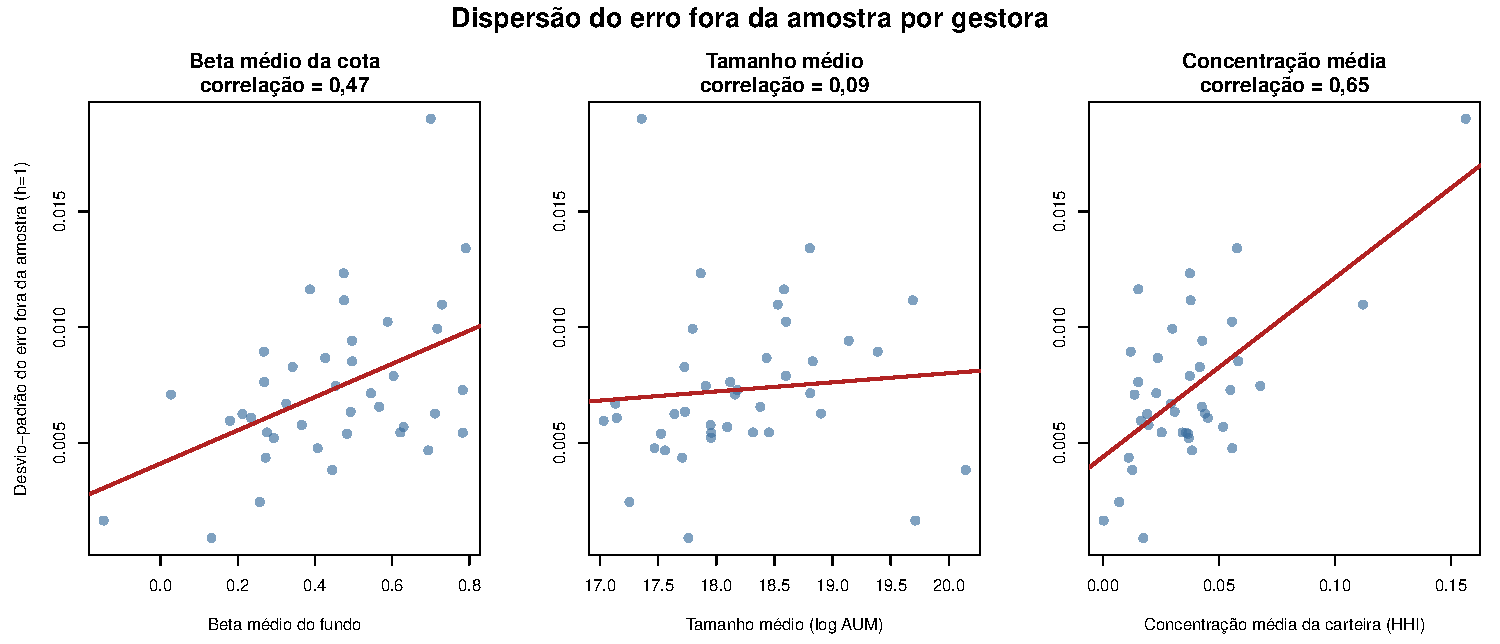
\includegraphics[width=0.95\textwidth]{fig_explica_variancia_gestora.pdf}
\caption{Desvio-padrão do erro por gestora vs.\ beta médio, tamanho médio, $\text{HHI}_{\text{medio}}$,
40 gestoras. Fonte: script \texttt{87\_explica\_variancia\_gestora.R}.}
\label{fig:explica-variancia}
\end{figure}

\begin{table}[h]\centering\small
\caption{Regressão múltipla (equação~\eqref{eq:regressao-variancia}): desvio-padrão do erro fora
da amostra por gestora explicado pelas 5 características não-HHI da Etapa 1 mais
$\text{HHI}_{\text{medio}}$, todas do período de treino. 40 gestoras. Fonte: script
\texttt{95\_regressao\_completa\_variancia.R}.}
\label{tab:regressao-variancia}
\begin{tabular}{@{}lrrc@{}}
\toprule
Variável & Coeficiente & $t$ & Sig. \\
\midrule
Intercepto ($\alpha$) & $-0{,}0147$ & $-1{,}32$ & n.s. \\
Beta médio do fundo & $0{,}0018$ & $0{,}73$ & n.s. \\
Tamanho médio, log AUM & $0{,}0010$ & $1{,}57$ & n.s. \\
Cotistas médio, log & $0{,}00002$ & $0{,}04$ & n.s. \\
\% FIC & $-0{,}0007$ & $-0{,}39$ & n.s. \\
Fluxo/AUM médio & $-0{,}0095$ & $-1{,}42$ & n.s. \\
$\text{HHI}_{\text{medio}}$ & $0{,}0840$ & $4{,}17$ & *** \\
\midrule
$R^2$ & \multicolumn{3}{r}{$0{,}545$} \\
\bottomrule
\end{tabular}
\caption*{\footnotesize $^{***}p<0{,}1\%$; n.s.\ = não significativo a $5\%$. Praticamente idêntica
à versão sem HHI na Etapa 1 ($R^2=0{,}54$, mesmo coeficiente/$t$ do HHI): HHI já estar na Etapa 1
não elimina seu poder explicativo aqui --- são perguntas diferentes.}
\end{table}

\paragraph{Concentração no nível fundo-mês.} Refinando para o nível fundo-mês (não mais média por
gestora): correlação contemporânea $0{,}42$ (Spearman $0{,}80$), defasada (mês $t-1$) $0{,}43$
(Spearman $0{,}80$) --- quase idênticas, afastando coincidência de mesmo mês --- e dentro do
fundo (demeaned) $0{,}06$ (Spearman $0{,}10$): a concentração é, sobretudo, um traço que
diferencia fundos entre si, não um sinal de curto prazo dentro do mesmo fundo.

\begin{figure}[H]\centering
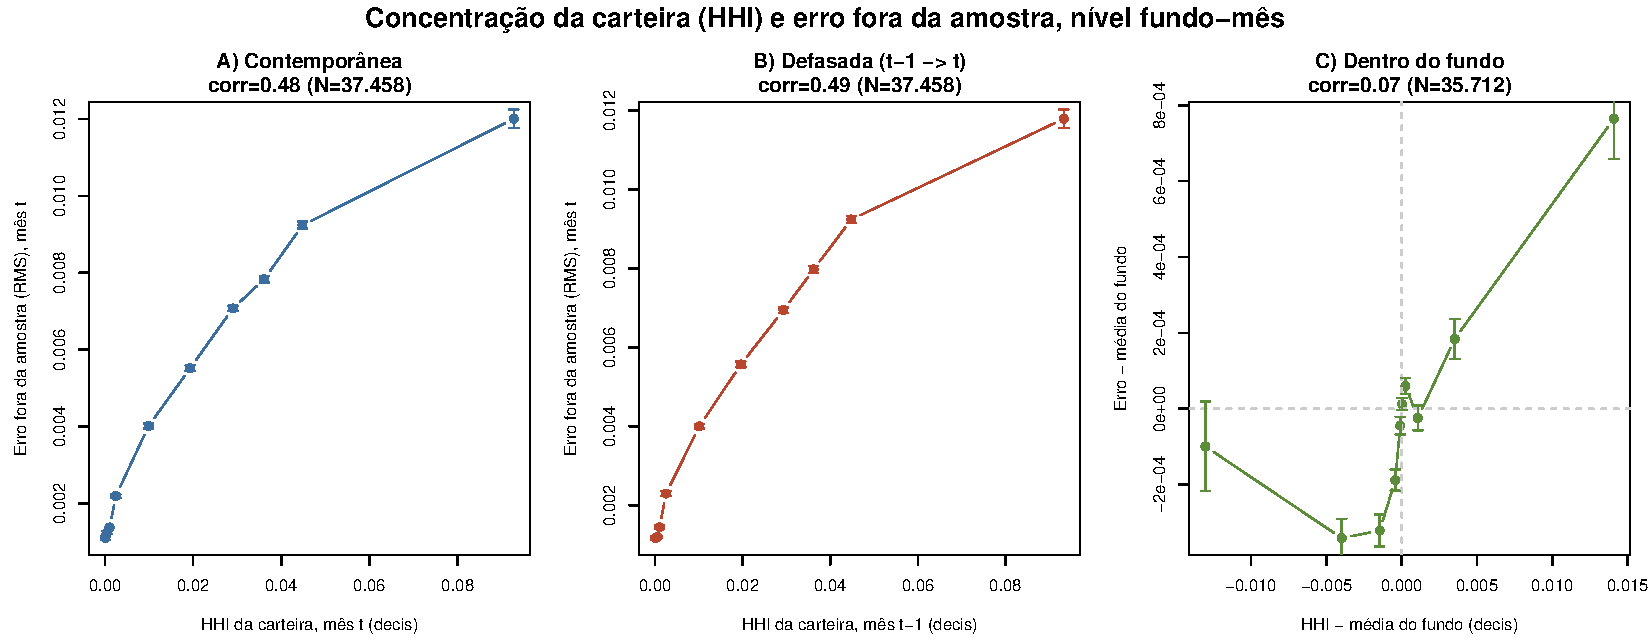
\includegraphics[width=0.95\textwidth]{fig_concentracao_mes_a_mes.pdf}
\caption{Concentração (HHI) vs.\ erro fora da amostra, nível fundo-mês, em decis. (A)
contemporânea; (B) defasada; (C) dentro do fundo. Fonte: script
\texttt{88\_concentracao\_mes\_a\_mes.R}.}
\label{fig:concentracao-mes}
\end{figure}

\begin{figure}[H]\centering
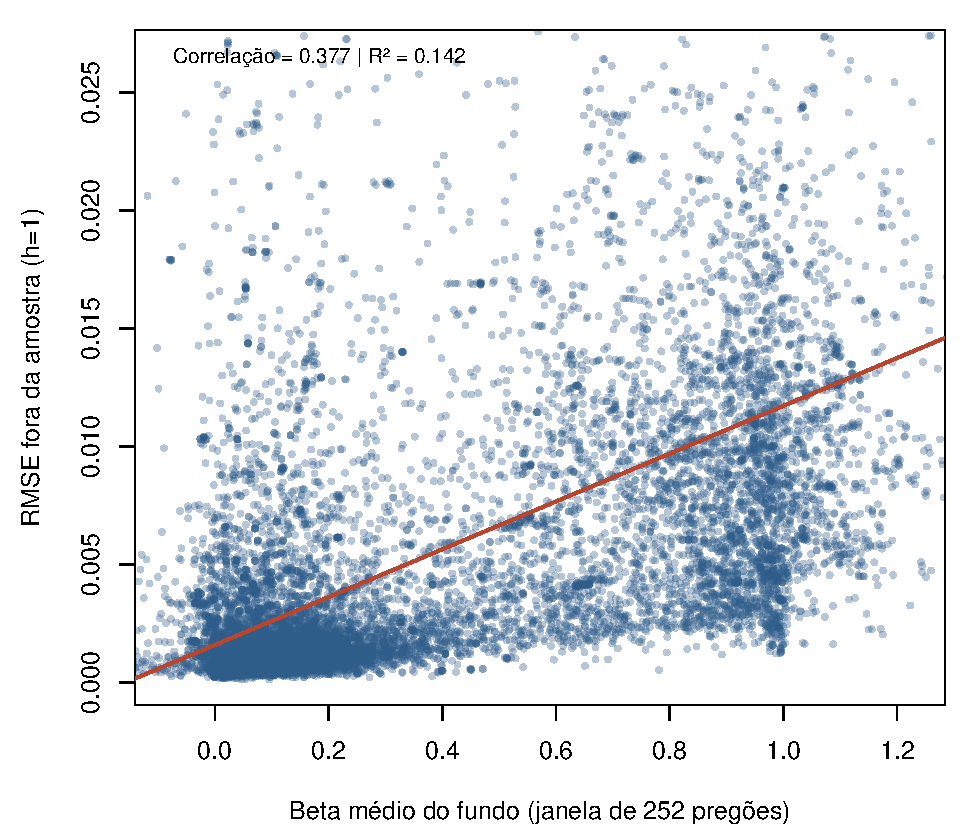
\includegraphics[width=0.68\textwidth]{fig_beta_vs_erro.pdf}
\caption{Beta médio do fundo vs.\ RMSE fora da amostra, 1.941 fundos ($\geq 6$ obs.\ de teste,
peso mediano $\geq 0{,}1\%$). $R^2=0{,}24$ (coef.\ $0{,}00749$, $p<10^{-100}$). Fonte: script
\texttt{78\_figura\_beta\_vs\_erro.R}.}
\label{fig:beta-erro}
\end{figure}

\begin{figure}[H]\centering
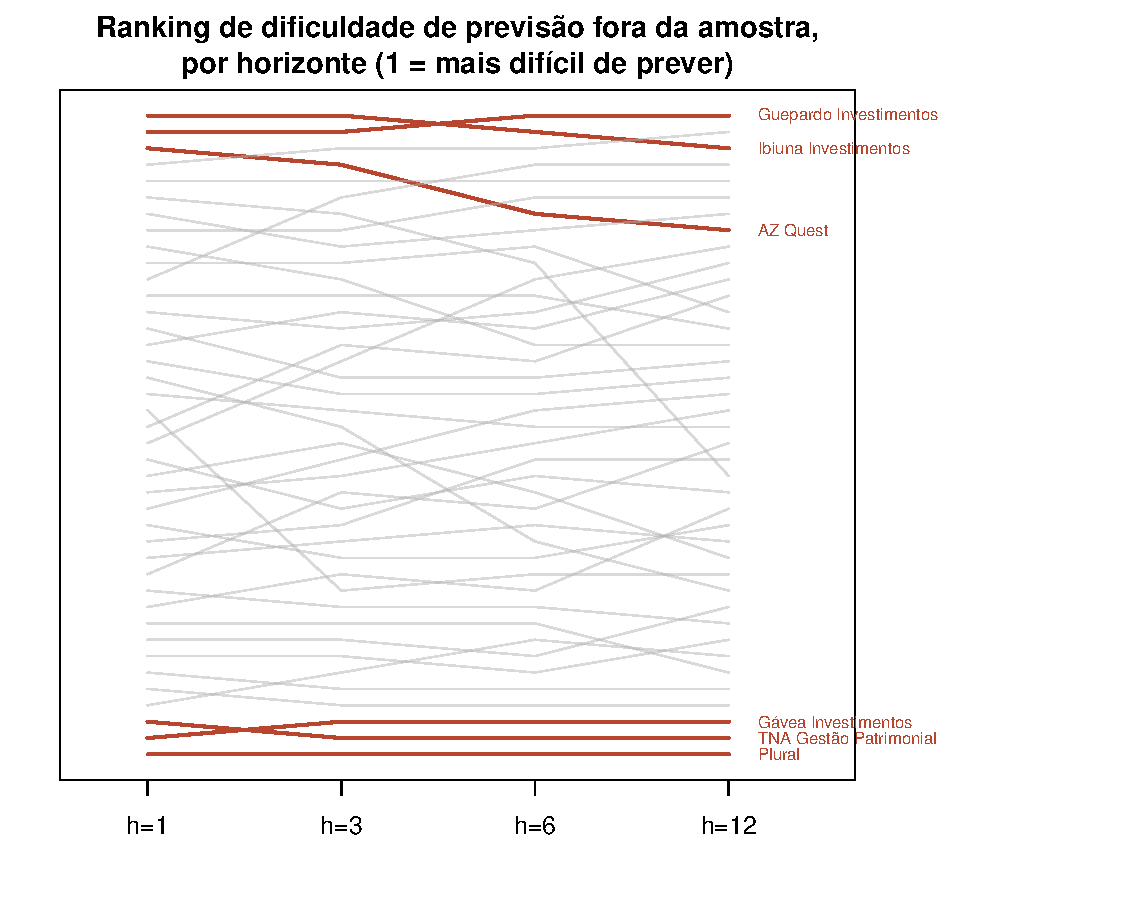
\includegraphics[width=0.75\textwidth]{fig_ranking_horizontes_slopegraph.pdf}
\caption{Estabilidade do ranking de dificuldade por gestora entre horizontes, 40 gestoras.
Spearman: $0{,}97$ ($h1$–$h3$), $0{,}94$ ($h1$–$h6$), $0{,}91$ ($h1$–$h12$), $0{,}98$
($h3$–$h6$), $0{,}95$ ($h3$–$h12$), $0{,}98$ ($h6$–$h12$). Fonte: script
\texttt{80\_figura\_ranking\_horizontes.R}.}
\label{fig:ranking-horizontes}
\end{figure}

\begin{center}\scriptsize
\begin{longtable}{@{}lrrrrr@{}}
\caption{RMSE fora da amostra por gestora, 4 horizontes, ordenado do mais ao menos errante em
$h=1$. Fonte: script \texttt{93\_gera\_latex\_tabelas\_9\_10.R} $\to$
\texttt{etapa3\_multiativo\_gestora\_multihorizonte.csv}.}
\label{tab:rmse-gestora}\\
\toprule
Gestora & Fundos ($h{=}1$) & RMSE $h{=}1$ & RMSE $h{=}3$ & RMSE $h{=}6$ & RMSE $h{=}12$ \\
\midrule
\endfirsthead
\multicolumn{6}{l}{\textit{(continuação)}}\\
\toprule
Gestora & Fundos ($h{=}1$) & RMSE $h{=}1$ & RMSE $h{=}3$ & RMSE $h{=}6$ & RMSE $h{=}12$ \\
\midrule
\endhead
\midrule
\multicolumn{6}{r}{\textit{continua na próxima página}}\\
\endfoot
\bottomrule
\endlastfoot
Ibiuna Investimentos & 7 & $0{,}01474$ & $0{,}02355$ & $0{,}02743$ & $0{,}03345$ \\
Guepardo Investimentos & 10 & $0{,}01428$ & $0{,}02325$ & $0{,}03380$ & $0{,}05651$ \\
AZ Quest & 22 & $0{,}01094$ & $0{,}01453$ & $0{,}01636$ & $0{,}01844$ \\
Núcleo Capital & 17 & $0{,}01043$ & $0{,}01830$ & $0{,}02497$ & $0{,}03583$ \\
Squadra Investimentos & 14 & $0{,}01008$ & $0{,}01397$ & $0{,}01695$ & $0{,}02160$ \\
Forpus Capital & 3 & $0{,}00951$ & $0{,}01372$ & $0{,}01555$ & $0{,}01559$ \\
Truxt Investimentos & 31 & $0{,}00809$ & $0{,}01254$ & $0{,}01587$ & $0{,}01938$ \\
Legacy Capital & 1 & $0{,}00805$ & --- & --- & --- \\
Sharp Capital & 34 & $0{,}00803$ & $0{,}01298$ & $0{,}01709$ & $0{,}02130$ \\
ARX Investimentos & 12 & $0{,}00791$ & $0{,}01083$ & $0{,}01260$ & $0{,}01515$ \\
Kinea Investimentos & 4 & $0{,}00717$ & $0{,}01158$ & $0{,}01504$ & $0{,}01537$ \\
Constellation Asset Management & 26 & $0{,}00693$ & $0{,}01378$ & $0{,}01844$ & $0{,}02775$ \\
Opportunity & 19 & $0{,}00677$ & $0{,}01050$ & $0{,}01346$ & $0{,}01582$ \\
Atmos Capital & 28 & $0{,}00613$ & $0{,}01000$ & $0{,}01337$ & $0{,}01692$ \\
SPX Capital & 35 & $0{,}00612$ & $0{,}00911$ & $0{,}01156$ & $0{,}01302$ \\
Verde Asset Management & 14 & $0{,}00601$ & $0{,}01023$ & $0{,}01298$ & $0{,}01650$ \\
Daycoval Asset Management & 5 & $0{,}00581$ & $0{,}00729$ & $0{,}00737$ & $0{,}00776$ \\
Absolute Investimentos & 7 & $0{,}00561$ & $0{,}00864$ & $0{,}01091$ & $0{,}01304$ \\
JGP & 40 & $0{,}00554$ & $0{,}00772$ & $0{,}00893$ & $0{,}01072$ \\
Kapitalo Investimentos & 22 & $0{,}00537$ & $0{,}00579$ & $0{,}00690$ & $0{,}00827$ \\
Bogari Capital & 14 & $0{,}00533$ & $0{,}00936$ & $0{,}01213$ & $0{,}01610$ \\
Credit Suisse & 65 & $0{,}00502$ & $0{,}00698$ & $0{,}00823$ & $0{,}00931$ \\
Real Investor & 5 & $0{,}00488$ & $0{,}00904$ & $0{,}01425$ & $0{,}01781$ \\
Claritas Investimentos & 10 & $0{,}00480$ & $0{,}00705$ & $0{,}00787$ & $0{,}00838$ \\
Caixa & 27 & $0{,}00461$ & $0{,}00682$ & $0{,}00888$ & $0{,}01141$ \\
Western Asset & 26 & $0{,}00436$ & $0{,}00698$ & $0{,}00958$ & $0{,}01248$ \\
Bradesco Asset Management & 277 & $0{,}00430$ & $0{,}00600$ & $0{,}00717$ & $0{,}00850$ \\
Vinci Partners & 48 & $0{,}00423$ & $0{,}00644$ & $0{,}00756$ & $0{,}00849$ \\
BB Asset Management & 103 & $0{,}00413$ & $0{,}00642$ & $0{,}00805$ & $0{,}00988$ \\
Occam Brasil & 26 & $0{,}00411$ & $0{,}00667$ & $0{,}00760$ & $0{,}00994$ \\
BTG Pactual & 139 & $0{,}00391$ & $0{,}00587$ & $0{,}00688$ & $0{,}00855$ \\
Santander Brasil Asset Management & 70 & $0{,}00391$ & $0{,}00541$ & $0{,}00623$ & $0{,}00727$ \\
Safra Asset Management & 136 & $0{,}00340$ & $0{,}00481$ & $0{,}00572$ & $0{,}00641$ \\
BNP Paribas & 42 & $0{,}00302$ & $0{,}00440$ & $0{,}00537$ & $0{,}00718$ \\
XP & 87 & $0{,}00292$ & $0{,}00442$ & $0{,}00529$ & $0{,}00737$ \\
Julius Baer Family Office & 57 & $0{,}00261$ & $0{,}00363$ & $0{,}00450$ & $0{,}00550$ \\
Itaú & 440 & $0{,}00260$ & $0{,}00384$ & $0{,}00466$ & $0{,}00548$ \\
Dahlia Capital & 18 & $0{,}00247$ & $0{,}00425$ & $0{,}00554$ & $0{,}00623$ \\
TNA Gestão Patrimonial & 29 & $0{,}00151$ & $0{,}00219$ & $0{,}00282$ & $0{,}00389$ \\
Gávea Investimentos & 17 & $0{,}00144$ & $0{,}00265$ & $0{,}00362$ & $0{,}00467$ \\
Plural & 1 & $0{,}00050$ & $0{,}00081$ & $0{,}00105$ & $0{,}00137$ \\
\end{longtable}
\end{center}

\begin{center}\scriptsize
\begin{longtable}{@{}lrrrr@{}}
\caption{Margem do ajuste parcial sobre a ingênua ($\%$ de redução de RMSE), mesma ordem da
Tabela~\ref{tab:rmse-gestora}. Negativo = ajuste parcial pior que a ingênua. Fonte: script
\texttt{93\_gera\_latex\_tabelas\_9\_10.R}.}
\label{tab:margem-gestora}\\
\toprule
Gestora & Margem $h{=}1$ & Margem $h{=}3$ & Margem $h{=}6$ & Margem $h{=}12$ \\
\midrule
\endfirsthead
\multicolumn{5}{l}{\textit{(continuação)}}\\
\toprule
Gestora & Margem $h{=}1$ & Margem $h{=}3$ & Margem $h{=}6$ & Margem $h{=}12$ \\
\midrule
\endhead
\midrule
\multicolumn{5}{r}{\textit{continua na próxima página}}\\
\endfoot
\bottomrule
\endlastfoot
Ibiuna Investimentos & $3{,}7\%$ & $8{,}1\%$ & $8{,}5\%$ & $15{,}0\%$ \\
Guepardo Investimentos & $0{,}9\%$ & $0{,}1\%$ & $-0{,}7\%$ & $-1{,}3\%$ \\
AZ Quest & $3{,}4\%$ & $7{,}5\%$ & $10{,}6\%$ & $16{,}4\%$ \\
Núcleo Capital & $-1{,}4\%$ & $-3{,}0\%$ & $-3{,}1\%$ & $-7{,}3\%$ \\
Squadra Investimentos & $0{,}6\%$ & $0{,}0\%$ & $-1{,}0\%$ & $-2{,}8\%$ \\
Forpus Capital & $1{,}9\%$ & $5{,}9\%$ & $8{,}9\%$ & $17{,}7\%$ \\
Truxt Investimentos & $1{,}7\%$ & $4{,}0\%$ & $6{,}3\%$ & $14{,}2\%$ \\
Legacy Capital & $-11{,}8\%$ & --- & --- & --- \\
Sharp Capital & $1{,}3\%$ & $4{,}2\%$ & $8{,}3\%$ & $15{,}0\%$ \\
ARX Investimentos & $2{,}1\%$ & $4{,}3\%$ & $6{,}9\%$ & $7{,}5\%$ \\
Kinea Investimentos & $2{,}3\%$ & $4{,}3\%$ & $10{,}0\%$ & $12{,}3\%$ \\
Constellation Asset Management & $-0{,}8\%$ & $-0{,}2\%$ & $2{,}5\%$ & $3{,}4\%$ \\
Opportunity & $1{,}6\%$ & $4{,}1\%$ & $6{,}8\%$ & $9{,}9\%$ \\
Atmos Capital & $0{,}1\%$ & $2{,}7\%$ & $5{,}2\%$ & $12{,}5\%$ \\
SPX Capital & $2{,}9\%$ & $7{,}3\%$ & $11{,}8\%$ & $20{,}1\%$ \\
Verde Asset Management & $0{,}4\%$ & $1{,}4\%$ & $2{,}9\%$ & $-0{,}7\%$ \\
Daycoval Asset Management & $3{,}5\%$ & $6{,}5\%$ & $8{,}8\%$ & $14{,}5\%$ \\
Absolute Investimentos & $1{,}7\%$ & $4{,}1\%$ & $6{,}9\%$ & $6{,}4\%$ \\
JGP & $2{,}3\%$ & $4{,}2\%$ & $4{,}8\%$ & $8{,}3\%$ \\
Kapitalo Investimentos & $3{,}0\%$ & $6{,}2\%$ & $7{,}5\%$ & $7{,}7\%$ \\
Bogari Capital & $-1{,}0\%$ & $-0{,}6\%$ & $0{,}0\%$ & $-5{,}4\%$ \\
Credit Suisse & $2{,}6\%$ & $5{,}1\%$ & $8{,}3\%$ & $15{,}2\%$ \\
Real Investor & $-2{,}4\%$ & $-0{,}1\%$ & $0{,}8\%$ & $6{,}1\%$ \\
Claritas Investimentos & $1{,}8\%$ & $6{,}2\%$ & $11{,}4\%$ & $19{,}1\%$ \\
Caixa & $1{,}8\%$ & $4{,}1\%$ & $7{,}0\%$ & $9{,}8\%$ \\
Western Asset & $1{,}0\%$ & $3{,}0\%$ & $5{,}4\%$ & $5{,}8\%$ \\
Bradesco Asset Management & $2{,}0\%$ & $3{,}7\%$ & $4{,}8\%$ & $4{,}3\%$ \\
Vinci Partners & $0{,}8\%$ & $3{,}0\%$ & $6{,}8\%$ & $18{,}7\%$ \\
BB Asset Management & $1{,}1\%$ & $2{,}6\%$ & $3{,}7\%$ & $4{,}9\%$ \\
Occam Brasil & $2{,}3\%$ & $5{,}0\%$ & $8{,}1\%$ & $10{,}6\%$ \\
BTG Pactual & $1{,}5\%$ & $2{,}8\%$ & $4{,}1\%$ & $5{,}0\%$ \\
Santander Brasil Asset Management & $2{,}0\%$ & $4{,}2\%$ & $5{,}7\%$ & $7{,}2\%$ \\
Safra Asset Management & $2{,}1\%$ & $3{,}4\%$ & $5{,}6\%$ & $9{,}2\%$ \\
BNP Paribas & $0{,}3\%$ & $-0{,}6\%$ & $-2{,}4\%$ & $-4{,}9\%$ \\
XP & $-2{,}9\%$ & $-6{,}2\%$ & $-10{,}2\%$ & $-12{,}3\%$ \\
Julius Baer Family Office & $1{,}5\%$ & $3{,}0\%$ & $4{,}8\%$ & $7{,}1\%$ \\
Itaú & $2{,}0\%$ & $4{,}6\%$ & $6{,}6\%$ & $8{,}4\%$ \\
Dahlia Capital & $2{,}3\%$ & $5{,}7\%$ & $8{,}6\%$ & $11{,}0\%$ \\
TNA Gestão Patrimonial & $-0{,}3\%$ & $-2{,}0\%$ & $-2{,}2\%$ & $1{,}0\%$ \\
Gávea Investimentos & $1{,}9\%$ & $4{,}2\%$ & $8{,}3\%$ & $11{,}2\%$ \\
Plural & $-3{,}2\%$ & $-5{,}4\%$ & $-4{,}7\%$ & $-8{,}5\%$ \\
\end{longtable}
\end{center}

\begin{figure}[h]\centering
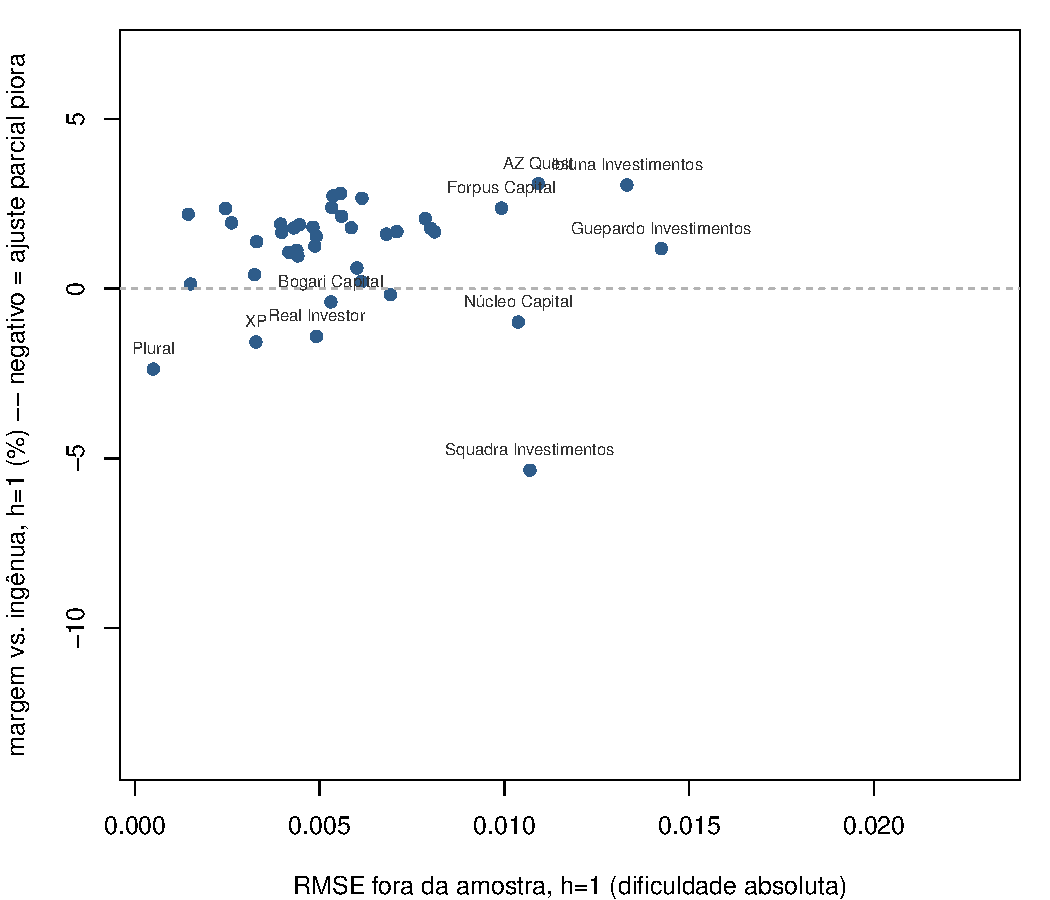
\includegraphics[width=0.7\textwidth]{fig_multihorizonte_gestora_rmse_margem.pdf}
\caption{Cada ponto é uma gestora: RMSE ($h{=}1$, eixo $x$) vs.\ margem sobre a ingênua ($h{=}1$,
eixo $y$; negativo = ajuste parcial piora). Fonte: script
\texttt{45\_fig\_multihorizonte\_gestora\_rmse\_margem.R}.}
\end{figure}

% ======================================================================
\FloatBarrier
\section{Aplicação}
\label{sec:aplicacao}

\emph{[Seção ainda incerta quanto à inclusão no TCC, conforme indicação do orientador.
Descreve uma estratégia --- apelidada internamente de ``robô caça-replicantes'' --- que usa a
estrutura do erro fora da amostra (Seção~\ref{sec:resultados}) para identificar pares de fundos
cujo erro se move em sincronia além do que suas características observáveis explicam.]}

% ======================================================================
\FloatBarrier
\section{Conclusão}

\emph{[Seção a ser escrita após a Introdução. Deve mencionar HHI\_resto como parte do modelo
final (Etapa 1, equação~\eqref{eq:hhi-resto}), não como extensão em avaliação.]}

\end{document}
